\problemname{The Dark Chambers of Chalmers}
You are on your way to the final competition of the Swedish Olympiad in Informatics, which is hosted at Chalmers Technical University.
However, you have gotten lost in the university basement.
Your sense of direction is not great, and what makes matters worse is the very strange design of the basement.

\begin{centering}
  \begin{figure}[h]
    \centering
    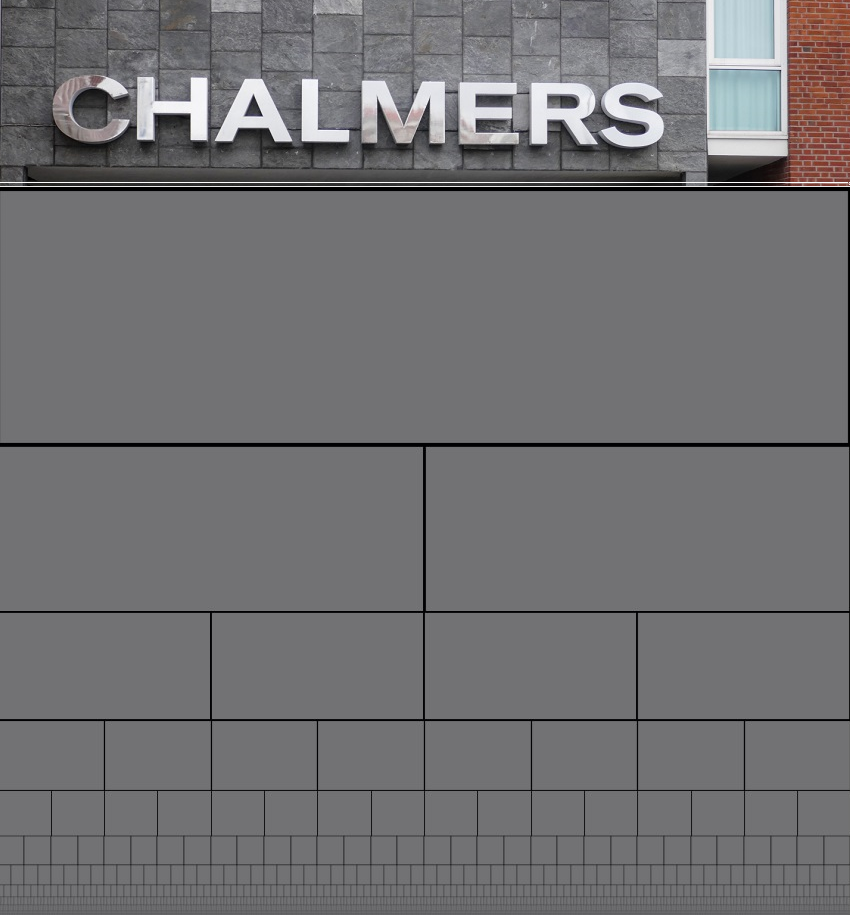
\includegraphics[scale=0.6]{chalmers_dark_chambers.png}
    \caption{The Dark Chambers of Chalmers...}
  \end{figure}
\end{centering}

The basement consists of $2 \leq N \leq 1000$ floors.
At the ground level, there is just one large room.
For all other rooms, there is some room directly above.
When you go down one floor, the rooms are half as big.
Beneath every room $i$, there are up to two rooms $l_i$ and $r_i$, each exactly half as big as room $i$.
It is possible that only one of $l_i$ and $r_i$ exists, or that both or neither of them exist.
You can move between two rooms through a door if they are directly next to each other,
or through a staircase if one room is directly above the other.
You are currently in some room in the basement, and you know that the final is also hosted somewhere in the basement.

A \emph{path} is a sequence of steps to adjacent rooms.
For some path $v$ from the room you are currently in to the room where the final is hosted,
let $A_v$ be the number of times you go through a door,
and $B_v$ be the number of times you go up or down a staircase.
The \emph{length} of a path is defined as the sum $L_v = A_v + B_v$.
You now want to get to the final competition. 
To aid you, you have downloaded the app Campus Maps.
Campus Maps is programmed to find the length of the path to your destination,
where the number of staircases you need to go up or down is minimized.
Of all possible paths $v$ to the room where the final is hosted the app will find all those that minimize the value of $B_v$.
Out of these paths, it will choose the one that minimizes the value of $L_v$.
It will then give you the value of $L_v$, the length of this path. 

Since the app is quite slow, you only have time to check it at most $500$ times.
You also do not have time to go to another room more than $5000$ times.


\begin{centering}
  \begin{figure}[h]
      \centering
      \begin{subfigure}
        \centering
        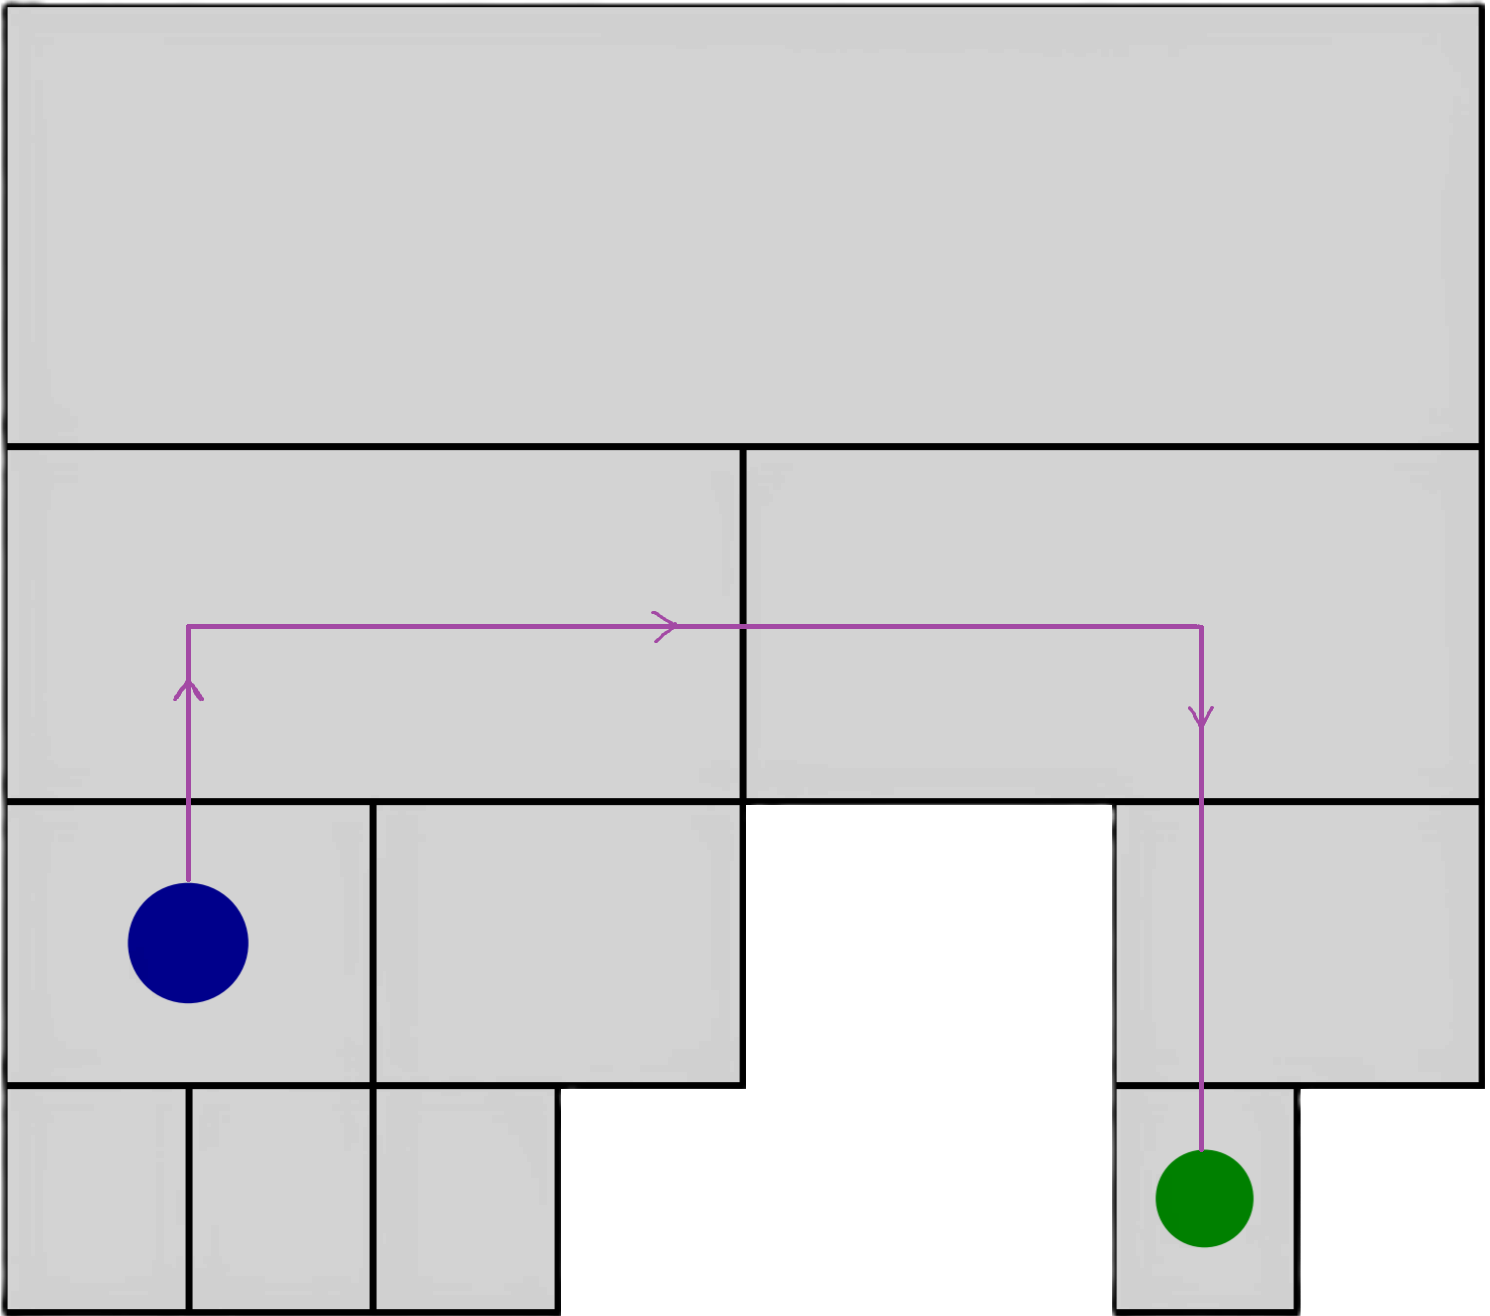
\includegraphics[scale=0.8]{sample1.png}
      \end{subfigure}
      \begin{subfigure}
        \centering
        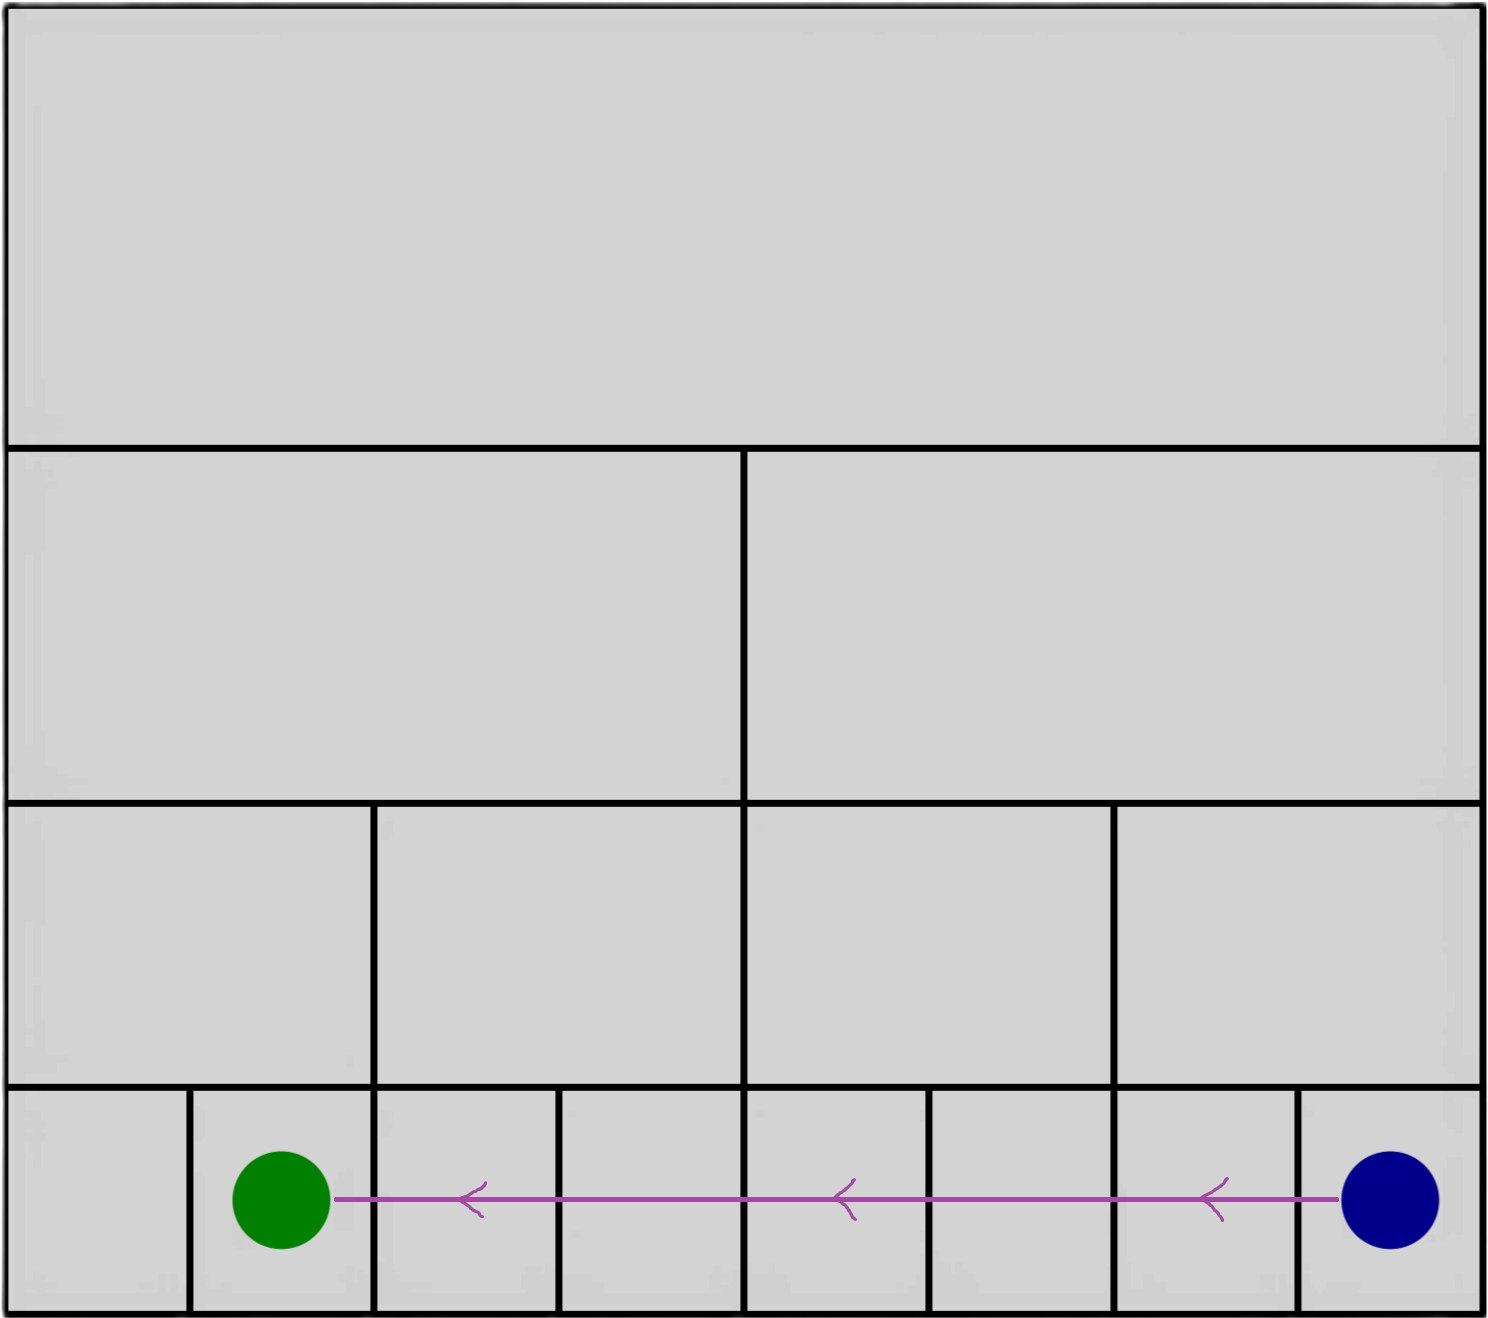
\includegraphics[scale=0.8]{sample2.png}
      \end{subfigure}
      \centering
      \caption{The basement in sample cases 1 and 2.
      The blue circle is your starting position, and the green circle shows which room the final is hosted in.
      In both images, the path that Campus Maps finds is illustrated in purple.
      In sample case 1, this path passes through three staircases and one door.
      In sample case 2, this path passes through zero staircases and six doors.
      }
      \label{fig:samples}
  \end{figure}
\end{centering}


\section*{Interaction}
First, you get information about the room you are currently in. 
This will be given as a binary string of length five, where every character is ``\texttt{1}'' if you can go in a certain direction, and ``\texttt{0}'' otherwise.
In order, the characters tell you if you can go up, right, down to the right, down to the left, and left.
So the string \texttt{01001} means that you can go to the right and to the left, but in no other directions.

Then, you choose either to go to an adjacent room, or to use Campus Maps.
To go to an adjacent room you write any of the strings 
``\texttt{up}'', ``\texttt{right}'', ``\texttt{downright}'', ``\texttt{downleft}'' or ``\texttt{left}''.
Then you get information about the new room you are in, according to the same format as above.

To use the app you write ``\texttt{app}''.
The app will then calculate the length of the shortest path from where you are to the goal that uses as few staircases as possible.
Since the app is very sensitive to Integer Overflows, it will crash if this length exceeds $10^9$.
In that case, the app will write $-1$.
Otherwise, the length of the path to the goal is written.

When you reach your destination, you should print out ``\texttt{here}'', and your program should be terminated.


\textbf{Make sure to flush the output after each query}, otherwise you can get \textit{Time Limit Exceeded}.
In C++ this can be done using \texttt{cout << flush;}
or \texttt{fflush(stdout);}
in Python with \texttt{stdout.flush()},
and in Java with \texttt{System.out.flush();}.

\section*{Scoring}
Your solution will be tested on a number of sample groups.
To get points in a group your solution must pass all test cases in that group.


\noindent
\begin{tabular}{| l | l | l |}
  \hline
  Group & Point value & Constraints \\ \hline \hline
  $1$   & $5$        & $N = 2$ \\ \hline
  $2$   & $10$        & $N \leq 10$ \\ \hline
  $3$   & $10$        & $N \leq 250$ \\ \hline
  $4$   & $16$        & Every room that is not on the lowest floor has two rooms directly below it. \\ \hline
  $4$   & $13$        & $N \leq 500$ \\ \hline
  $5$   & $21$        & $N \leq 950$ \\ \hline
  $6$   & $25$        & $N \leq 1000$ \\ \hline
\end{tabular}
